\documentclass[11pt]{article}

\hoffset        2mm 
\voffset        -15mm
\oddsidemargin  0mm
\topmargin      0.5in
\textwidth      6in
\textheight     9in

\usepackage{graphicx}
\usepackage{amsmath}
\usepackage[labelfont=bf,font=small]{caption}
\usepackage{float}
\usepackage{mhchem}

\usepackage{placeins}
\usepackage{makecell}

\usepackage{pdfpages}

\usepackage{chngcntr}
\counterwithin*{equation}{section}

\usepackage[toc,page]{appendix}

\begin{document}

\begin{titlepage}

\vspace*{55mm}
\begin{center}
{\huge deal.II ifpack Interface for BoomerAMG use as a Solver or Preconditioner}\\[1cm]
{\em \huge Math 676 Project Report \\ May 2019}\\[17mm]
\end{center}

\begin{flushright}
{\LARGE Joshua Hanophy}
\end{flushright}

\vfill

 \date{\today}

\end{titlepage}
\newpage
\tableofcontents
\newpage
\section{Introduction}

The \textit{hypre} library includes a variety of high performance preconditioners and solvers that are able to function in massively parallel applications \cite{hypre_description}. In practice, this means that all algorithms and data structures have been designed to exhibit reasonable parallel scaling in complexity and memory requirements. One important consequence of this from the perspective of a finite element program using \textit{hypre} is that data structures like the problem mesh, solution and forcing vector, and the global matrix that grow as the problem grows must be distributed among the processors being used to solve the problem in parallel. Distributed means that each processor stores only a portion of the total data structure. Obviously, no processor can know about the entire mesh or global matrix in a massively parallel simulation, because each processor has access to only a finite amount of memory to store data and a problem can be made arbitrarily large such that the memory requirements exceed storage capacity.

The deal.II finite element library includes the ability to setup and solve problems using massively parallel systems \cite{deal.ii}. For distributed data structures and distributed linear algebra, deal.II relies on separate libraries. For domain decomposition and storage of a fully distributed mesh, deal.II relies on the p4est library \cite{p4est}. For fully distributed matrices and vectors, deal.II can use petsc or Trilinos. The Trilinos library was used in the program constructed as part of this project \cite{Trilinos_general}. Trilinos can interface with \textit{hypre} in several ways. For this project, the ifpack package was used \cite{ifpack-guide}.

Algebraic multigrid (AMG) methods have been widely used to solve systems arising from the discretization of elliptic partial differential equations. In serial, AMG algorithms scale linearly with problem size. In parallel, communication costs scale logarithmically with the number of processors \cite{falgout1}. Recently, a classical AMG method based on approximate ideal restriction (AIR) was developed for nonsymmetric matrices. AIR has already been shown to be effective for solving the linear systems arising from upwind discontinuous Galerkin (DG) finite element discretization of advection-diffusion problems, including the hyperbolic limit of pure advection \cite{AIR1}\cite{AIR2}. A new parallel version of AIR, pAIR, has been implemented in the \textit{hypre} library.

Currently, there is no interface in deal.II to \textit{hypre} through Trilinos. The goal of this project was to created an interface to \textit{hypre} using ifpack. The interface will:
\begin{itemize}
	\item Allow for access to BoomerAMG as either a solver or a preconditioner for one of the other solvers in \textit{hypre}
	\item Include useful defaults for both Classical AMG and the new AIR AMG
	\item Inculde the functionality to easily adjust or add AMG parameters
\end{itemize}

The interface created for this project is fully documented with Doxygen. The Doxygen generated documentation is included as Appendix. The overal design is briefly described in this introduction as well. There are a significant number of parameters that can be used to control the operation of BoomerAMG. These parameters can have several known types. These types include double, int, or int *, as well as several others. Boost::variant was used to store items related to the parameters. This is a container that can hold different types. The types the container can hold are declared statically and so if an incorrect type is placed in the container, this error can be caught at compile time. All parameters are stored in a map with a string key. Helper functions to change parameters values, add new parameters, and delete parameters were all added. 

Three different programs were created to demonstrate the interface. These three programs are described in more detail in subsequent sections. 

\section{SUPG Test Program}
The advection diffusion problem shown in Equation \ref{advection_diffusion_strong} is of interest in this section. When this equation is discretized using the Galerkin method with continuous one dimensional elements, the results discretized system can be shown to be analogous to a discretization using central difference \cite{fem_for_flow_problems}. The truncation error associated with central differencing the advection term subtracts from the diffusion coefficient. When the velocity is sufficiently high enough, the actual diffusion coefficient can become negative. This problem with central differencing leads to instability.

Stabilization techniques add diffusion in various ways to cancel out the contribution from the central difference truncation error. In this section a program that implements an SUPG discritization is described. The SUPG discretization implemented in described in \cite{fem_for_flow_problems}. First, the weak formulation of Equation \ref{advection_diffusion_strong} is shown in Equation \ref{advection_diffusion_weak} $w=0$ on $\Gamma_D$ where $\Gamma_D$ is the portion of the boundary with Dirichlet conditions.

\begin{equation}
\label{advection_diffusion_strong}
\vec{a} \cdot \nabla u - \nabla \cdot \left( \nu \nabla u \right) = s
\end{equation}

\begin{equation}
\begin{aligned}
\label{advection_diffusion_weak}
\int_\Omega w\left( \vec{a} \cdot \nabla u \right)d\Omega +&\int_\Omega \nabla w \cdot \nu \nabla u d\Omega\\
&= \int_\Omega  wsd\Omega \;\;\; \forall w\in V
\end{aligned}
\end{equation}

The SUPG discretization is a consistent stabilization technique. First, the residual is defined as shown in Equation \ref{supg_residual}. Then the stabilization is added as shown in Equation \ref{sup_weak_with_stabil} where $\mathcal{P}(w)$ and $\tau$ are defined below. $h_\eta$ and $h_\xi$ are characteristic lengths whose values are defined in \cite{fem_for_flow_problems}.

\begin{equation}
\label{supg_residual}
\mathcal{R}(u) = \vec{a} \cdot \nabla u - \nabla \cdot \left( \nu \nabla u \right) - s
\end{equation}

\begin{equation}
\label{sup_weak_with_stabil}
a(w,u) + c(\vec{a};w,v) + \sum_e \int_{\Omega^e}\mathcal{P}(w)\tau \mathcal{R}(u)=(w,s)
\end{equation}

\begin{equation}
\mathcal{P}(w) = \vec{a} \cdot \nabla w
\end{equation}

\begin{equation}
\tau = \frac{\bar{\nu}}{||a||^2}
\end{equation}

\begin{equation}
\bar{\nu}=\frac{1}{2}\left( \bar{\xi} a_\xi h_\xi + \bar{\eta} a_\eta h_\eta \right)
\end{equation}

Shown below are definitions related to $\xi$, analogous definitions exist for $\eta$. $\xi$ and $\eta$ are coordinates in the natural coordinate system

\begin{equation}
\begin{aligned}
&\bar{\xi} = \coth Pe_\xi - \frac{1}{Pe_\xi} \\
&Pe_\xi = a_\xi h_\xi / (2\nu) \\
&a_\xi = \vec{e}_\xi \cdot \vec{a}
\end{aligned}
\end{equation}

The SUPG test program constructed includes the option so solve a problem with or without stabilization. Additionally, three different solvers can be used. These are the AIR AMG solver, the Classical AMG solver, or the direct Trilinos solver already implemented in deal.II. The program currently only works in two-dimension and with linear elements. The stabilization would have to be adjusted to work in three dimensions or with higher order elements. Also, in the current program, AMR has been disabled and uniform mesh refinement is currently being used instead for simplicity.

\subsection{Results}
Figure \ref{fig:no_supg_natural} and Figure \ref{fig:supg_natural} both show results with natural boundary conditions which here mean natural for an advection diffusion problem. The inflow boundary is set with a homogeneous Dirichlet condition and the outflow boundary condition is set with a homogeneous Neumann boundary condition. In this case, there is negligible difference between the stabilized result and the non stabilized result.

Figure \ref{fig:no_supg_dir} and Figure \ref{fig:supg_dir} show simulation results with homogeneous Dirichlet boundary conditions. In this case, the unstabilized results oscillates severely towards the outflow face of the problem. The stabilized version is not completely smooth, but is much smoother by comparison.  


\begin{figure}[ht]
	\centering
	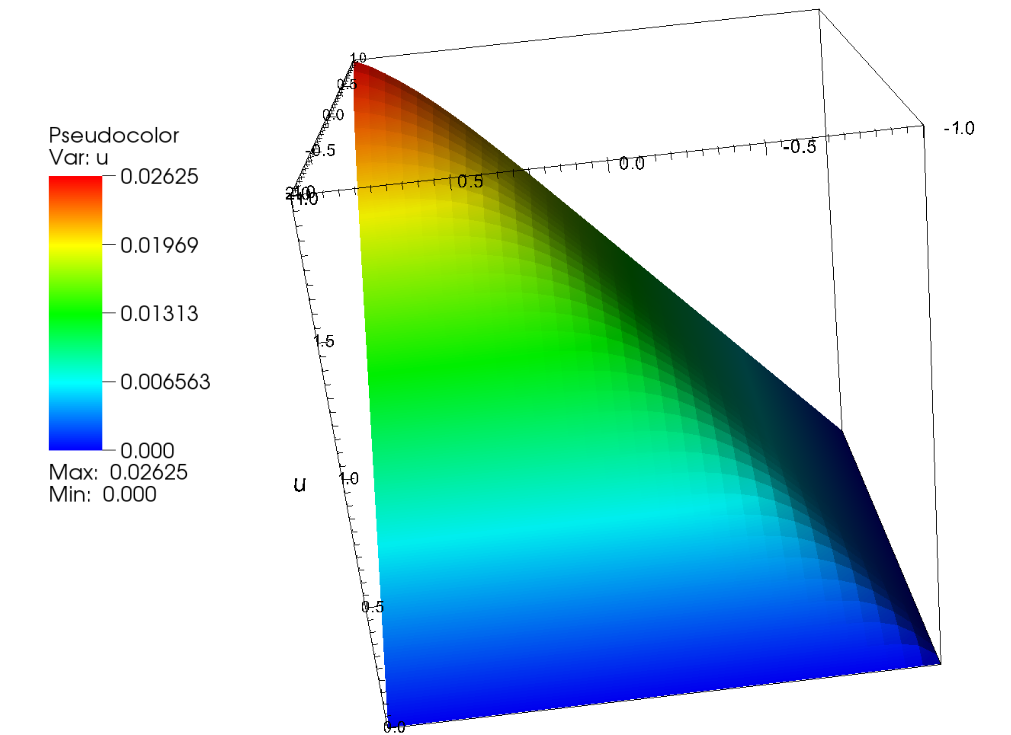
\includegraphics[scale=0.3]{./figures/no_supg_natural.png}
	\caption{Natural boundary conditions without stabilization.}
	\label{fig:no_supg_natural}
\end{figure}

\begin{figure}[ht]
	\centering
	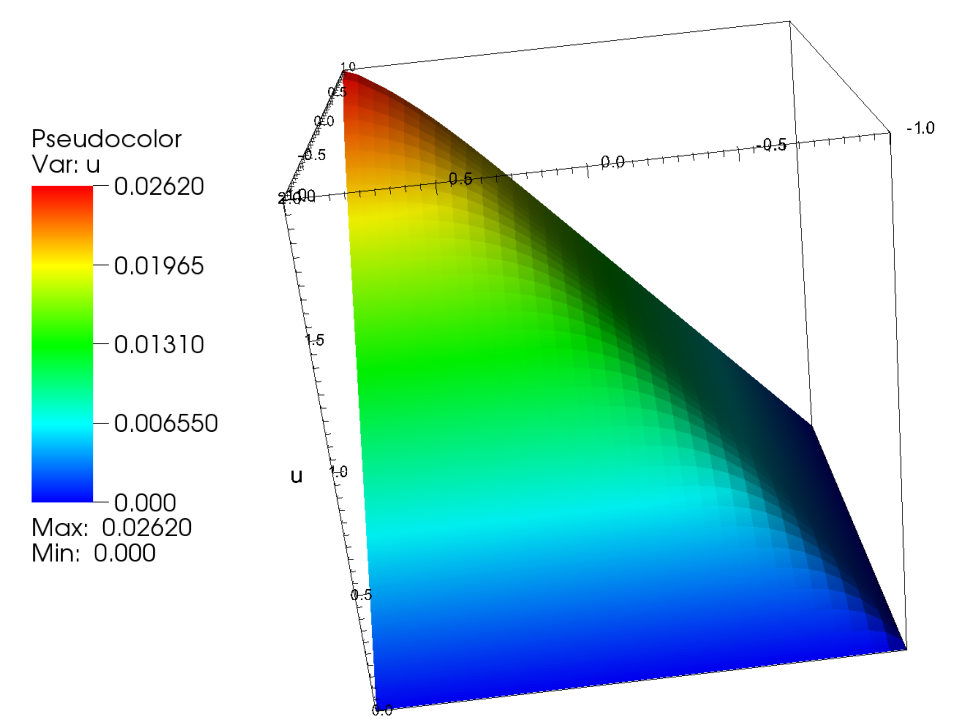
\includegraphics[scale=0.3]{./figures/supg_natural.png}
	\caption{Natural boundary conditions with stabilization.}
	\label{fig:supg_natural}
\end{figure}

\begin{figure}[ht]
	\centering
	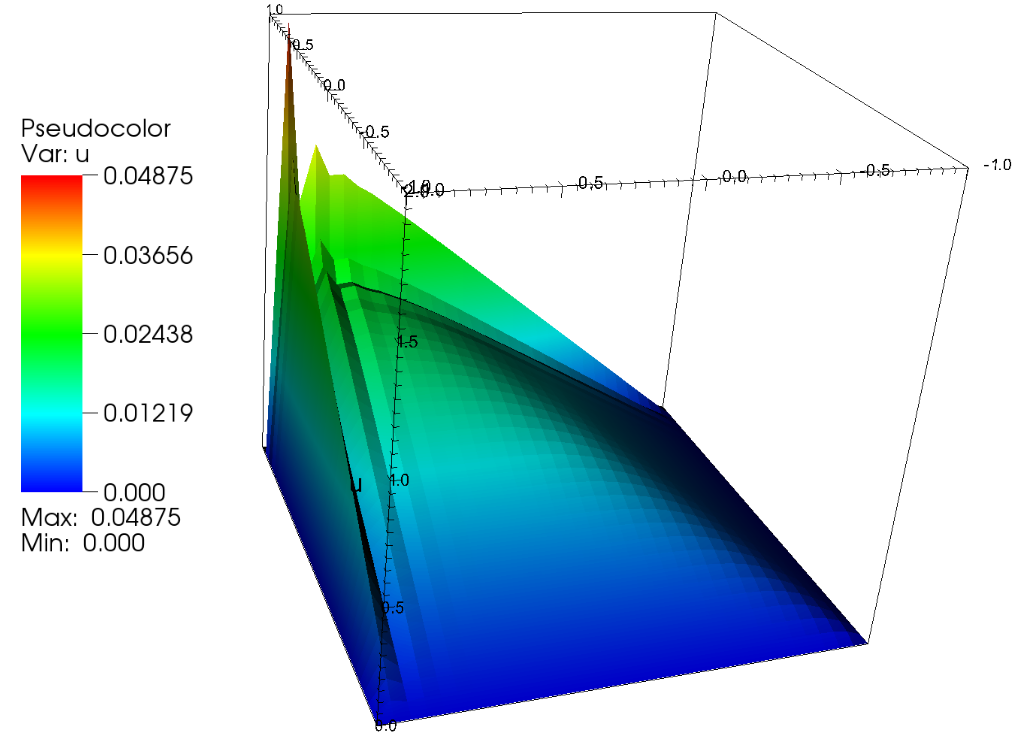
\includegraphics[scale=0.3]{./figures/no_supg_dir.png}
	\caption{Homogeneous Dirichlet boundary conditions without stabilization}
	\label{fig:no_supg_dir}
\end{figure}

\begin{figure}[ht]
	\centering
	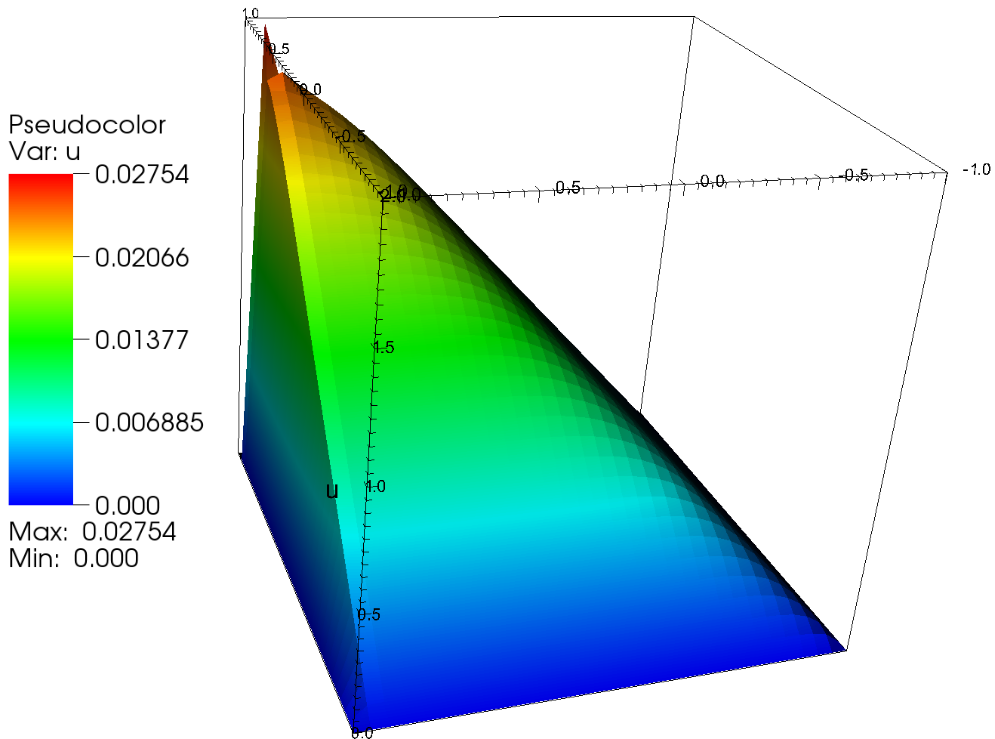
\includegraphics[scale=0.3]{./figures/supg_dir.png}
	\caption{Homogeneous Dirichlet boundary conditions with stabilization}
	\label{fig:supg_dir}
\end{figure}

\FloatBarrier
\subsection{Solving with AMG}
When the advection diffusion equation is discritized, the resulting system is not symmetric. Therefore, such a problem may be difficult for classical AMG to solve while being a good candidate for solution with AIR AMG. Table \ref{tab:supg_air_classical_comparison} shows the results for solving the system with AIR AMG and Classical AMG. Surprisingly, classical AMG works well for this problem. More investigation into this is required.

\begin{table}[!h]
	\begin{center}
		\label{tab:supg_air_classical_comparison}
		\caption{Result from stabilized SUPR problem with homogeneous Dirichlet boundary conditions and 265,240 cells. The problem was run in parallel on four processors.}
		\begin{tabular}{|c|c|c|}
			\hline
			Solver & Average Convergence Factor & Total Time \\ \hline
			\makecell{Classic Interpolation\\based AMG}&0.10&3.44 s \\ \hline
			\makecell{AIR AMG}&0.31&5.96 s \\ \hline
		\end{tabular}
	\end{center}
\end{table}

\section{Diffusion Test Program}
The interface created for this project includes the ability to use BoomerAMG as a preconditioner to another solver in \textit{hypre} or as a solver. To demonstrate the interfaces and test functionality, a program was created that solves diffusion. The program was partially based off of the tutorial step 40 program. Several different solvers were tested. These were the Conjugate Gradient (CG), Incomplete Cholesky Decomposition preconditioned CG (IC PCG), BoomerAMG preconditioned CG, ML Preconditioned CG, and BoomerAMG as a solver. This was not a rigorous evaluation, but provides some basic insights into performance. The converged tolerance of 1e-10 was used to generate all results. Additionally, only two dimensional results are presented here.

Table \ref{table:small_const_diff} and Table \ref{table:larger_const_diff} show results for solving diffusion with a constant diffusion coefficient. The AMG preconditioners as well as the AMG solvers all perform well. IC preconditioned CG and CG are performing poorly as for the larger problem. Table \ref{table:varying_diff} shows results for a problem where the diffusion coefficient varies discontinuously. The jump is from 100.0 to 0.001 and such a configuration will generally lead to a poorly conditioned matrix. CG does not converge for this problem within 3,000 iterations. The AMG preconditioned solvers as well as the AMG solver work effectively for this problem.  

\begin{table}[!h]
	\begin{center}
		\caption{Spatially constant diffusion coefficient for a problem with 1228 cells. The problem was run in parallel on four processors.}
		\label{table:small_const_diff}
		\begin{tabular}{|c|c|c|c|c|}
			\hline
			
			&\multicolumn{2}{c|}{\makecell{Linear\\Elements}} & \multicolumn{2}{c|}{\makecell{Quadratic\\Elements}} \\
			\cline{1-5}
			
			\textbf{Solver} & \textbf{Iterations} &\textbf{Time (s)}& \textbf{Iterations} &\textbf{Time (s)} \\\hline
			
			CG & 84 & 0.00366  & 223 & 0.0337 \\ \hline
			
			IC PCG & 69 & 0.00353  & 88 & 0.0229 \\ \hline
			
			BoomerAMG PCG& 8 & 0.00987 & 8 & 0.0236\\ \hline
			
			BoomerAMG as Solver & 14 & 0.00870 & 16 & 0.0280\\ \hline
			
			ML\_Epetra PCG &  11 & 0.00798 & 23 & 0.0412  \\ \hline
			
		\end{tabular}
	\end{center}
\end{table}

\begin{table}[!h]
	\begin{center}
		\caption{Spatially constant diffusion coefficient for a problem with 67093 cells. The problem was run in parallel on four processors.}
		\label{table:larger_const_diff}
		\begin{tabular}{|c|c|c|c|c|}
			\hline
			
			&\multicolumn{2}{c|}{\makecell{Linear\\Elements}} & \multicolumn{2}{c|}{\makecell{Quadratic\\Elements}} \\
			\cline{1-5}
			
			\textbf{Solver} & \textbf{Iterations} &\textbf{Time (s)}& \textbf{Iterations} &\textbf{Time (s)} \\\hline
			
			CG & 630 & 1.57  & 1735 & 28.2 \\ \hline
			
			IC PCG & 411 & 1.98  & 492 & 13.4 \\ \hline
			
			BoomerAMG PCG& 9 & 0.346 & 9 & 1.83\\ \hline
			BoomerAMG as Solver & 19 & 0.477 & 21 & 2.71\\ \hline
			
			ML\_Epetra PCG &  12 & 0.286 & 25 & 2.34  \\ \hline
			
		\end{tabular}
	\end{center}
\end{table}

\begin{table}[!h]
	\begin{center}
		\caption{Spatially varying discontinuous diffusion coefficient as shown in Figure \ref{fig:odd_diffusion} for a problem with 67093 cells. The problem was run in parallel on four processors.}
		\label{table:varying_diff}
		\begin{tabular}{|c|c|c|c|c|}
			\hline
			
			&\multicolumn{2}{c|}{\makecell{Linear\\Elements}} & \multicolumn{2}{c|}{\makecell{Quadratic\\Elements}} \\
			\cline{1-5}
			
			\textbf{Solver} & \textbf{Iterations} &\textbf{Time (s)}& \textbf{Iterations} &\textbf{Time (s)} \\\hline
			
			IC PCG & 589 & 2.49  & 731 & 18.3 \\ \hline
			
			BoomerAMG PCG& 8 & 0.347 & 9 & 1.91\\ \hline
			
			BoomerAMG as Solver & 17 & 0.456 & 20 & 2.62\\ \hline
			
			ML\_Epetra PCG &  15 & 0.308 & 36 & 3.02  \\ \hline
			
		\end{tabular}
	\end{center}
\end{table}

\begin{figure}[ht]
	\centering
	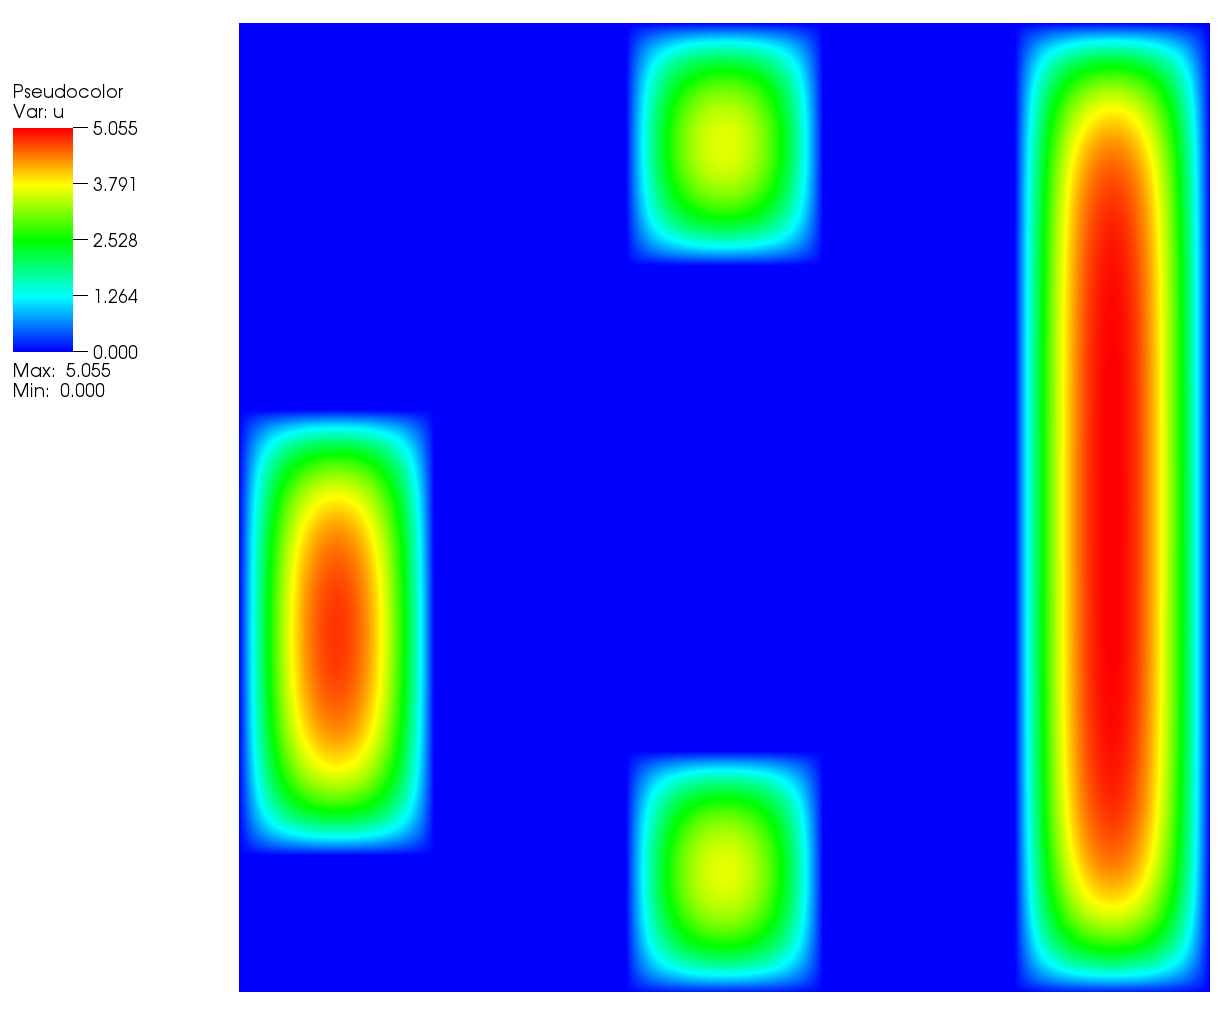
\includegraphics[scale=0.3]{./figures/odd_diffusion_config.png}
	\caption{Test diffusion problem created where the diffusion coefficient changes discontinuously in space}
	\label{fig:odd_diffusion}
\end{figure}

\FloatBarrier
\section{DG Advection in Parallel}
The deal.II tutorial program step 12 implements DG advection. The sample program in written to run on a single processor. The test AIR AMG as a solver, the step 12 tutorial program was changed to work in parallel and the AIR AMG solver was implemented. Figure \ref{fig:step_12_domain_decomp} shows the domain decomposition after step 12 was run in parallel on four processors. The AIR solver is able to solve the problem in parallel. No specific results are presented in this section, however, parallel scaling results for AIR as implemented in \textit{hypre} will be published in the near future.

\begin{figure}[ht]
	\centering
	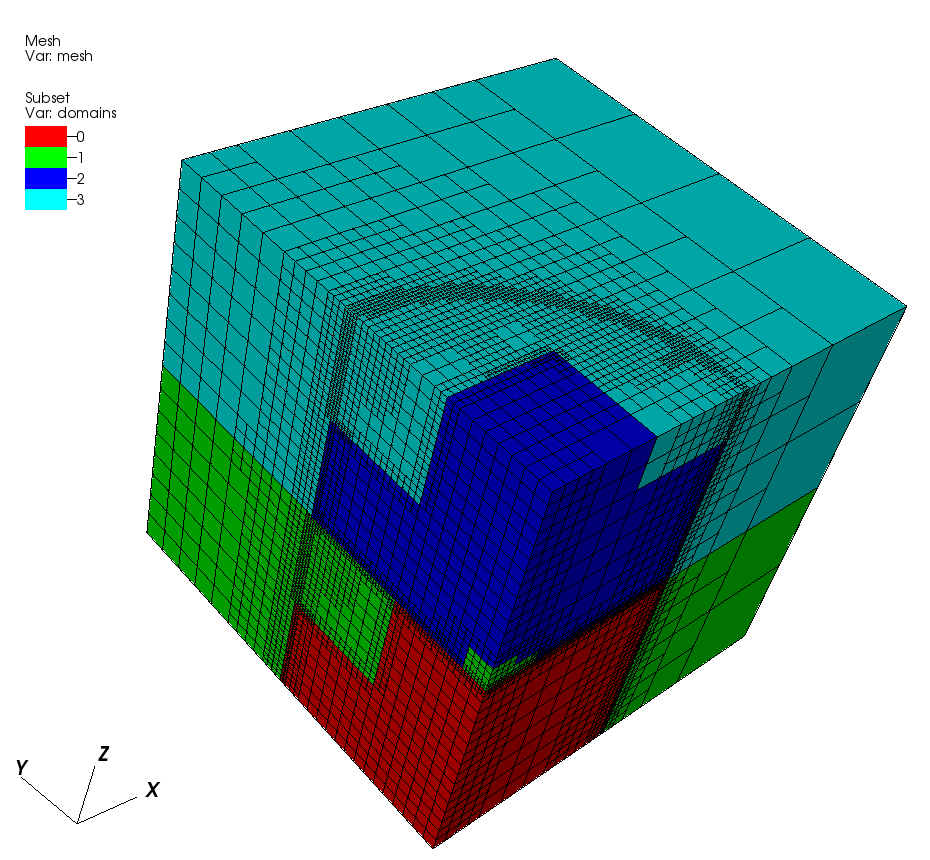
\includegraphics[scale=0.3]{./figures/step_12_parallel_domain_decomp.png}
	\caption{Domain decomposition after the step 12 problem was run in parallel on four processors.}
	\label{fig:step_12_domain_decomp}
\end{figure}


\FloatBarrier
\newpage
\begin{thebibliography}{9}

	\bibitem{hypre_description} 
	R.D. Falgout, J.E. Jones, and U.M. Yang. 
	The Design and Implementation of hypre, a Library of Parallel High Performance Preconditioners, chapter in Numerical Solution of Partial Differential Equations on Parallel Computers, A.M. Bruaset and A. Tveito, eds., Springer-Verlag, 51 (2006), pp. 267-294. UCRL-JRNL-205459.
	
   	\bibitem{deal.ii} 
	G. Alzetta, D. Arndt, W. Bangerth, V. Boddu, B. Brands, D. Davydov, R. Gassmoeller, T. Heister, L. Heltai, K. Kormann, M. Kronbichler, M. Maier, J.-P. Pelteret, B. Turcksin, and D. Wells. "The \textit{deal.II} Library, Version 9.0." \textit{Journal of Numerical Mathematics} (2018, accepted).	
	
	\bibitem{p4est} 
	C. Burstedde, L. C. Wilcox, and O. Ghattas. 
    "\textit{p4est}: Scalable Algorithms for Parallel Adaptive Mesh Refinement on Forests of Octrees." \textit{SIAM Journal on Scientific Computing}, \textbf{volume 33}(3), pp. 1103-1133 (2011).
    
	\bibitem{Trilinos_general} 
	M. A. Heroux, R. A. Bartlett, V. E. Howle, R. J. Hoekstra, J. J. Hu, T. G. Kolda, R. B. Lehoucq, K. R. Long, R. P. Pawlowski, E. T. Phipps, A. G. Salinger, H. K. Thornquist, R. S. Tuminaro, J. M. Willenbring, A. Williams, and K. S. Stanley, “An overview of the trilinos project,” ACM Trans. Math. Softw., vol. 31, no. 3, pp. 397–423, 2005.
	
	\bibitem{ifpack-guide}
	M. Sala and M. Heroux, “Robust algebraic preconditioners with IFPACK 3.0,” Tech. Rep. SAND-0662, Sandia National Laboratories, 2005.
	
	\bibitem{falgout1}
	R. Falgout. “An introduction to algebraic multigrid.” \textit{Computing in Science \& Engineering}, \textbf{volume 8}(6), pp. 24–33 (2009).
	
	\bibitem{AIR1}
	T. A. Manteuffel, S. F. McCormick, S. Munzenmaier, J. W. Ruge, and B. S. Southworth. “Reduction-based Algebraic Multgrid for Upwind Discretizations.” \textit{SIAM Journal on Scientific Computing} (submitted).
	
	\bibitem{AIR2}
	T. A. Manteuffel, J. W. Ruge, and B. S. Southworth. “Nonsymmetric Reduction-based Algebraic Multigrid Based on Local Approximate Ideal Restriction (LAIR).” \textit{SIAM Journal on Scientific Computing} (submitted).
	
	\bibitem{fem_for_flow_problems}
	J. Donea and A. Huerta. "Finite Element Methods for Flow Problems." John Wiley \& Sons Ltd, West Sussex, England, 2003.
	
\end{thebibliography}

\newpage
\begin{appendices}
	\chapter{Interface Doxygen Documentation}
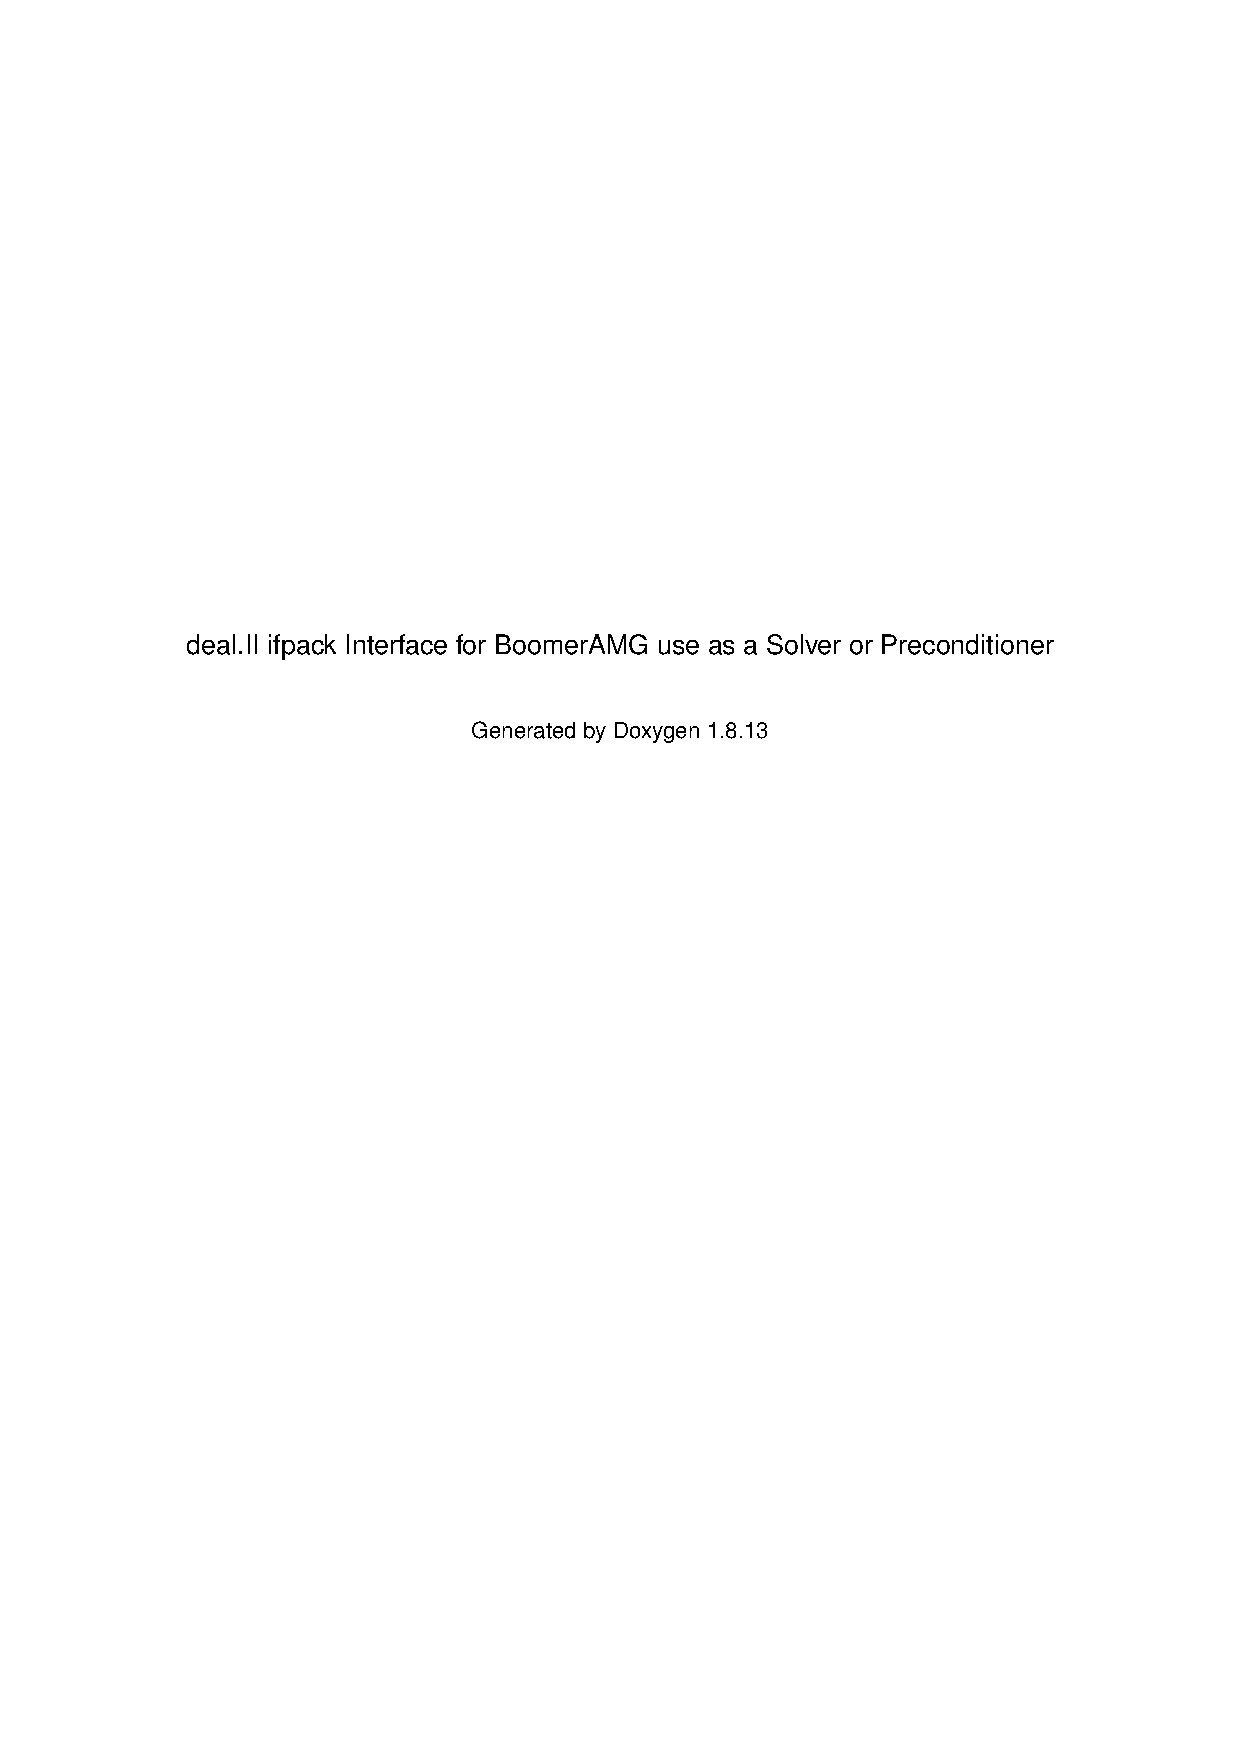
\includepdf[pages=-,offset=0 -10]{refman.pdf}
\end{appendices}

\end{document}








